\documentclass[tikz,border=5pt]{standalone}
\usepackage[T1]{fontenc}
\usepackage{lmodern}
\usepackage{pgf-pie}

% Muted extensions of the manuscript's existing red-blue palette.
\definecolor{errRubric}{HTML}{7A2430}
\definecolor{errScore}{HTML}{B45D68}
\definecolor{errFactual}{HTML}{174D68}
\definecolor{errEvidence}{HTML}{5E8497}
\definecolor{errUnsupported}{HTML}{3F7F77}
\definecolor{errContradiction}{HTML}{B08A57}
\definecolor{errIrrelevant}{HTML}{8A8194}

\definecolor{posFirst}{HTML}{7A2430}
\definecolor{posSecond}{HTML}{B45D68}
\definecolor{posThird}{HTML}{5E8497}
\definecolor{posLast}{HTML}{174D68}
\definecolor{legendRule}{HTML}{4A4A4A}
\definecolor{noteText}{HTML}{333333}
\tikzset{pie slice/.style={draw=white,line width=0.7pt}}

\newcommand{\legenditem}[3]{%
  \begin{scope}[shift={#2}]
    \fill[fill=#1, draw=legendRule, line width=0.3pt]
      (0,0) rectangle (0.24,0.24);
    \node[anchor=west, font=\sffamily\scriptsize]
      at (0.34,0.12) {#3};
  \end{scope}%
}

\begin{document}
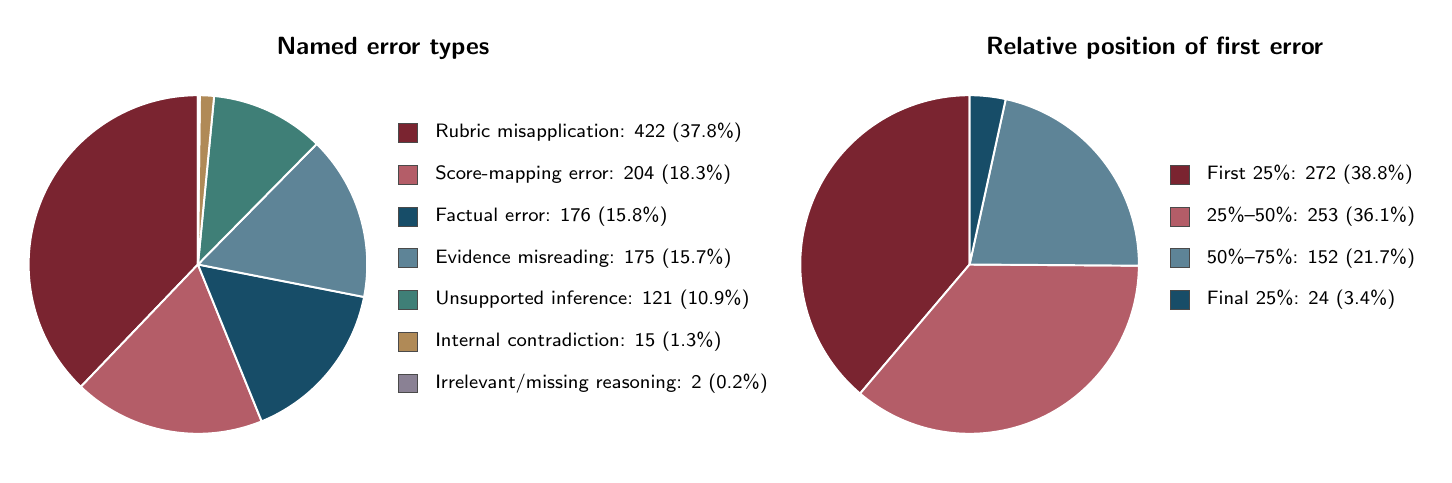
\begin{tikzpicture}[font=\sffamily]

% Panel (a): 1,115 sentences with an explicitly named error type.
\node[font=\sffamily\small\bfseries] at (2.35,2.75)
  {Named error types};
\begin{scope}[shift={(0,0)}]
  \pie[%
sum=1115,%
radius=2.15,%
rotate=90,%
hide number,%
text=inside,%
style=pie slice,%
color={errRubric,errScore,errFactual,errEvidence,errUnsupported,%
           errContradiction,errIrrelevant}%
  ]{422/,204/,176/,175/,121/,15/,2/}
\end{scope}

\legenditem{errRubric}{(2.55,1.55)}{Rubric misapplication: 422 (37.8\%)}
\legenditem{errScore}{(2.55,1.02)}{Score-mapping error: 204 (18.3\%)}
\legenditem{errFactual}{(2.55,0.49)}{Factual error: 176 (15.8\%)}
\legenditem{errEvidence}{(2.55,-0.04)}{Evidence misreading: 175 (15.7\%)}
\legenditem{errUnsupported}{(2.55,-0.57)}{Unsupported inference: 121 (10.9\%)}
\legenditem{errContradiction}{(2.55,-1.10)}{Internal contradiction: 15 (1.3\%)}
\legenditem{errIrrelevant}{(2.55,-1.63)}{Irrelevant/missing reasoning: 2 (0.2\%)}

% Panel (b): first-error locations in 701 harmful DS-to-RF cases.
\node[font=\sffamily\small\bfseries] at (12.15,2.75)
  {Relative position of first error};
\begin{scope}[shift={(9.8,0)}]
  \pie[%
sum=701,%
radius=2.15,%
rotate=90,%
hide number,%
text=inside,%
style=pie slice,%
color={posFirst,posSecond,posThird,posLast}%
  ]{272/,253/,152/,24/}
\end{scope}

\legenditem{posFirst}{(12.35,1.02)}{First 25\%: 272 (38.8\%)}
\legenditem{posSecond}{(12.35,0.49)}{25\%--50\%: 253 (36.1\%)}
\legenditem{posThird}{(12.35,-0.04)}{50\%--75\%: 152 (21.7\%)}
\legenditem{posLast}{(12.35,-0.57)}{Final 25\%: 24 (3.4\%)}

\end{tikzpicture}
\end{document}
